\subsection{AlphaNIST Training Framework}

\begin{figure*}[t]
    \centering
    \resizebox{\textwidth}{!}{\begin{tikzpicture}[
    x=1mm,
    y=1mm,
    font=\footnotesize\sffamily,
    flow/.style={-{Latex[length=1.8mm,width=1.15mm]}, draw=graphite,
        line width=0.5pt},
    source/.style={rounded corners=0.5mm, line width=0.45pt, align=center,
        inner sep=1.2mm},
    layer/.style={line width=0.4pt, minimum width=2.4mm,
        minimum height=10mm, inner sep=0pt, align=center},
    annotation/.style={font=\scriptsize\sffamily, text=graphite, align=center}
]
    \definecolor{graphite}{RGB}{48,55,59}
    \definecolor{geomblue}{RGB}{77,115,144}
    \definecolor{stateblue}{RGB}{91,142,131}
    \definecolor{networkblue}{RGB}{115,151,166}
    \definecolor{networkgold}{RGB}{169,136,41}
    \tikzset{every node/.style={text=graphite}}

    \node[source, draw=geomblue, fill=white, text width=29mm,
        minimum height=13mm] (geometry) at (15,12)
        {\textbf{Point cloud}};
    \node[source, draw=stateblue, fill=white, text width=33mm,
        minimum height=12mm] (history) at (17,-10)
        {\textbf{Proprioception + last action}\\[-1pt]
        pose $7$ $\mid$ twist $6$ $\mid$ joints $9$ $\mid$ action $8$};

    \node[layer, draw=geomblue, fill=geomblue!75]
        (pc-in) at (38,12) {};
    \node[layer, draw=geomblue, fill=geomblue!75]
        (pc-hidden) at (49,12) {};
    \node[layer, draw=geomblue, fill=geomblue!75]
        (pc-out) at (58,12) {};
    \node[annotation] at (48,21) {two-layer ELU encoder};
    \node[annotation, below=1.0mm of pc-in] {$3\times n_{\mathrm{pts}}$};
    \node[annotation, below=1.0mm of pc-hidden] {$256$};
    \node[annotation, below=1.0mm of pc-out] {$128$};
    \draw[flow] (geometry.east) -- (pc-in.west);
    \draw[flow] (pc-in.east) -- (pc-hidden.west);
    \draw[flow] (pc-hidden.east) -- (pc-out.west);

    \node[layer, draw=stateblue, fill=stateblue!75]
        (state-in) at (42,-10) {};
    \node[layer, draw=stateblue, fill=stateblue!35]
        (state-norm) at (50,-10) {};
    \node[annotation, above=1.0mm of state-norm] {RN};
    \node[layer, draw=stateblue, fill=stateblue!75]
        (state-out) at (58,-10) {};
    \node[annotation, below=1.0mm of state-in] {$150$};
    \node[annotation, below=1.0mm of state-out] {$150$};
    \draw[flow] (history.east) -- (state-in.west);
    \draw[flow] (state-in.east) -- (state-norm.west);
    \draw[flow] (state-norm.east) -- (state-out.west);

    \node[circle, draw=graphite, fill=white, line width=0.5pt,
        minimum size=7.5mm, inner sep=0pt] (concat) at (66,0) {$\Vert$};
    \node[annotation, below=1.0mm of concat] {$278$};
    \draw[flow] (pc-out.east) -- (concat.north west);
    \draw[flow] (state-out.east) -- (concat.south west);

    \foreach \branch/\yy in {actor/15,critic/-16} {
        \node[layer, draw=geomblue, fill=networkblue]
            (projection-\branch) at (76,\yy) {};
        \node[annotation, above=1.0mm of projection-\branch] {linear};
        \node[annotation, below=1.0mm of projection-\branch] {$256$};

        \foreach \block/\offset in {1/0,2/43} {
            \path[draw=graphite!28, fill=white,
                line width=0.35pt, rounded corners=0.65mm]
                ({80+\offset},{\yy-10}) rectangle ({120+\offset},{\yy+16});
            \coordinate (res-in-\branch-\block) at ({81+\offset},\yy);
            \node[layer, draw=stateblue, fill=stateblue!35]
                (layer-norm-\branch-\block) at ({86+\offset},\yy) {};
            \node[annotation, above=1.0mm of layer-norm-\branch-\block] {LN};
            \node[layer, draw=geomblue, fill=networkblue]
                (expand-\branch-\block) at ({93+\offset},\yy) {};
            \node[annotation, above=1.0mm of expand-\branch-\block] {linear};
            \node[annotation, below=1.0mm of expand-\branch-\block] {$1024$};
            \node[layer, draw=networkgold, fill=networkgold!45]
                (swish-\branch-\block) at ({100+\offset},\yy) {};
            \node[annotation, above=1.0mm of swish-\branch-\block] {SW};
            \node[layer, draw=geomblue, fill=networkblue]
                (contract-\branch-\block) at ({107+\offset},\yy) {};
            \node[annotation, above=1.0mm of contract-\branch-\block] {linear};
            \node[annotation, below=1.0mm of contract-\branch-\block] {$256$};
            \node[circle, draw=graphite, fill=white,
                line width=0.5pt, minimum size=5.5mm, inner sep=0pt]
                (res-add-\branch-\block) at ({116+\offset},\yy) {$+$};
            \draw[flow] (layer-norm-\branch-\block.east) -- (expand-\branch-\block.west);
            \draw[flow] (expand-\branch-\block.east) -- (swish-\branch-\block.west);
            \draw[flow] (swish-\branch-\block.east) -- (contract-\branch-\block.west);
            \draw[flow] (contract-\branch-\block.east) -- (res-add-\branch-\block.west);
            \draw[flow, rounded corners=0.8mm]
                (res-in-\branch-\block) -- ++(0,11mm) --
                node[above=0.4mm, annotation, fill=white, inner sep=0.4mm] {identity}
                ({116+\offset},{\yy+11}) -- (res-add-\branch-\block.north);
            \fill[graphite] (res-in-\branch-\block) circle[radius=0.4mm];
        }
        \draw[flow] (projection-\branch.east) -- (layer-norm-\branch-1.west);
        \draw[flow] (res-add-\branch-1.east) -- (layer-norm-\branch-2.west);

        \node[layer, draw=stateblue, fill=stateblue!35]
            (out-norm-\branch) at (168,\yy) {};
        \node[annotation, above=1.0mm of out-norm-\branch] {LN};
        \node[layer, draw=networkgold!85!black, fill=networkgold!80]
            (head-\branch) at (175,\yy) {};
        \draw[flow] (res-add-\branch-2.east) -- (out-norm-\branch.west);
        \draw[flow] (out-norm-\branch.east) -- (head-\branch.west);
    }

    \draw[flow, rounded corners=1mm]
        (concat.north east) |- (projection-actor.west);
    \draw[flow, rounded corners=1mm]
        (concat.south east) |- (projection-critic.west);

    \node[annotation, above=1.0mm of head-actor] {linear};
    \node[annotation, below=1.0mm of head-actor] {$8$};
    \foreach \j [evaluate=\j as \x using 182+(\j-1)*2.7] in {1,...,7} {
        \node[draw=networkgold!85!black, fill=networkgold!80, line width=0.45pt,
            rounded corners=0.15mm, minimum size=2.6mm, inner sep=0pt]
            (arm-\j) at (\x,15) {};
    }
    \node[draw=stateblue, fill=stateblue!75, line width=0.45pt,
        rounded corners=0.15mm, minimum size=2.6mm, inner sep=0pt]
        (gripper) at (203,15) {};
    \node[annotation, font=\scriptsize\sffamily\bfseries] at (192.5,20.2)
        {Gaussian action $a_t\in\mathbb{R}^{8}$};
    \draw[flow] (head-actor.east) -- (arm-1.west);
    \draw[draw=graphite, line width=0.4pt]
        ([yshift=-1mm]arm-1.south west) -- ++(0,-1mm) -|
        ([yshift=-1mm]arm-7.south east) -- ++(0,1mm);
    \node[annotation, text=graphite] at (190,9.6)
        {arm $\Delta q_{1:7}$};
    \node[annotation, text=graphite] at (203,9.6)
        {gripper};

    \node[annotation, above=1.0mm of head-critic] {linear};
    \node[annotation, below=1.0mm of head-critic] {$1$};
    \node[draw=networkgold!85!black, fill=networkgold!80, line width=0.45pt,
        rounded corners=0.15mm, minimum size=3.2mm, inner sep=0pt]
        (value-cell) at (182,-16) {};
    \node[annotation, font=\scriptsize\sffamily\bfseries,
        text=graphite, anchor=west] at (186,-16)
        {value $V_\phi(o_t)\in\mathbb{R}$};
    \draw[flow] (head-critic.east) -- (value-cell.west);
\end{tikzpicture}
}
    \caption{\textbf{Policy architecture.} 
    Actor and critic have the same architecture with separate
    parameters. Inputs are drawn once; each network contains two consecutive
    residual blocks. RN: running normalization; LN: layer normalization;
    SW: Swish activation; $n_{\mathrm{pts}}$: number of input points.}
    \label{fig:policy-architecture}
\end{figure*}



AlphaNIST trains one policy across all 20 assembly tasks with standard PPO
and a binary task reward for completed assembly.
Its training distribution combines diverse cached
reset states from OmniReset~\cite{yin2026omnireset} with beta-distributed success-guided sampling (SGS)~\cite{zhang2026balanceddiet}, while a common binary task
reward defines successful assembly across all tasks. The three components
play distinct roles:


\[
\begin{array}{r@{\quad}l}
\textbf{Reset bank:}    & \textit{Which states are available?}\\
\textbf{Beta sampling:} & \textit{Which states are sampled?}\\
\textbf{Binary task reward:} & \textit{What counts as success?}
\end{array}
\]




\subsection{Reset Coverage and Experience Allocation}
\label{sec:success_guided_sampling}


We adapt OmniReset~\cite{yin2026omnireset} to heterogeneous assembly by
caching the assembly identity together with each reset state:
\begin{equation}
    \mathcal{D}_{\mathrm{reset}}
    =\{(e_i,\bar{s}_i)\}_{i=1}^{M}.
\end{equation}
Here, $M$ is the total number of entries across all 20 assemblies.
The assembly identity $e_i$ selects the part and mating-geometry assets and their inertial properties, while $\bar{s}_i$ specifies the robot,
board, and movable-part state. Sampling an entry therefore selects
both the assembly and its initial configuration.
The cached bank spans ungrasped
workspace, pickup, transport, near-mating, and partially assembled
configurations (Fig.~\ref{fig:reset-coverage}), enabling GPU-parallel
initialization. These reset families
define regions of the training distribution, not a prescribed sequence; the
policy receives no stage identifier.

\begin{figure}[!tb]
    \centering
    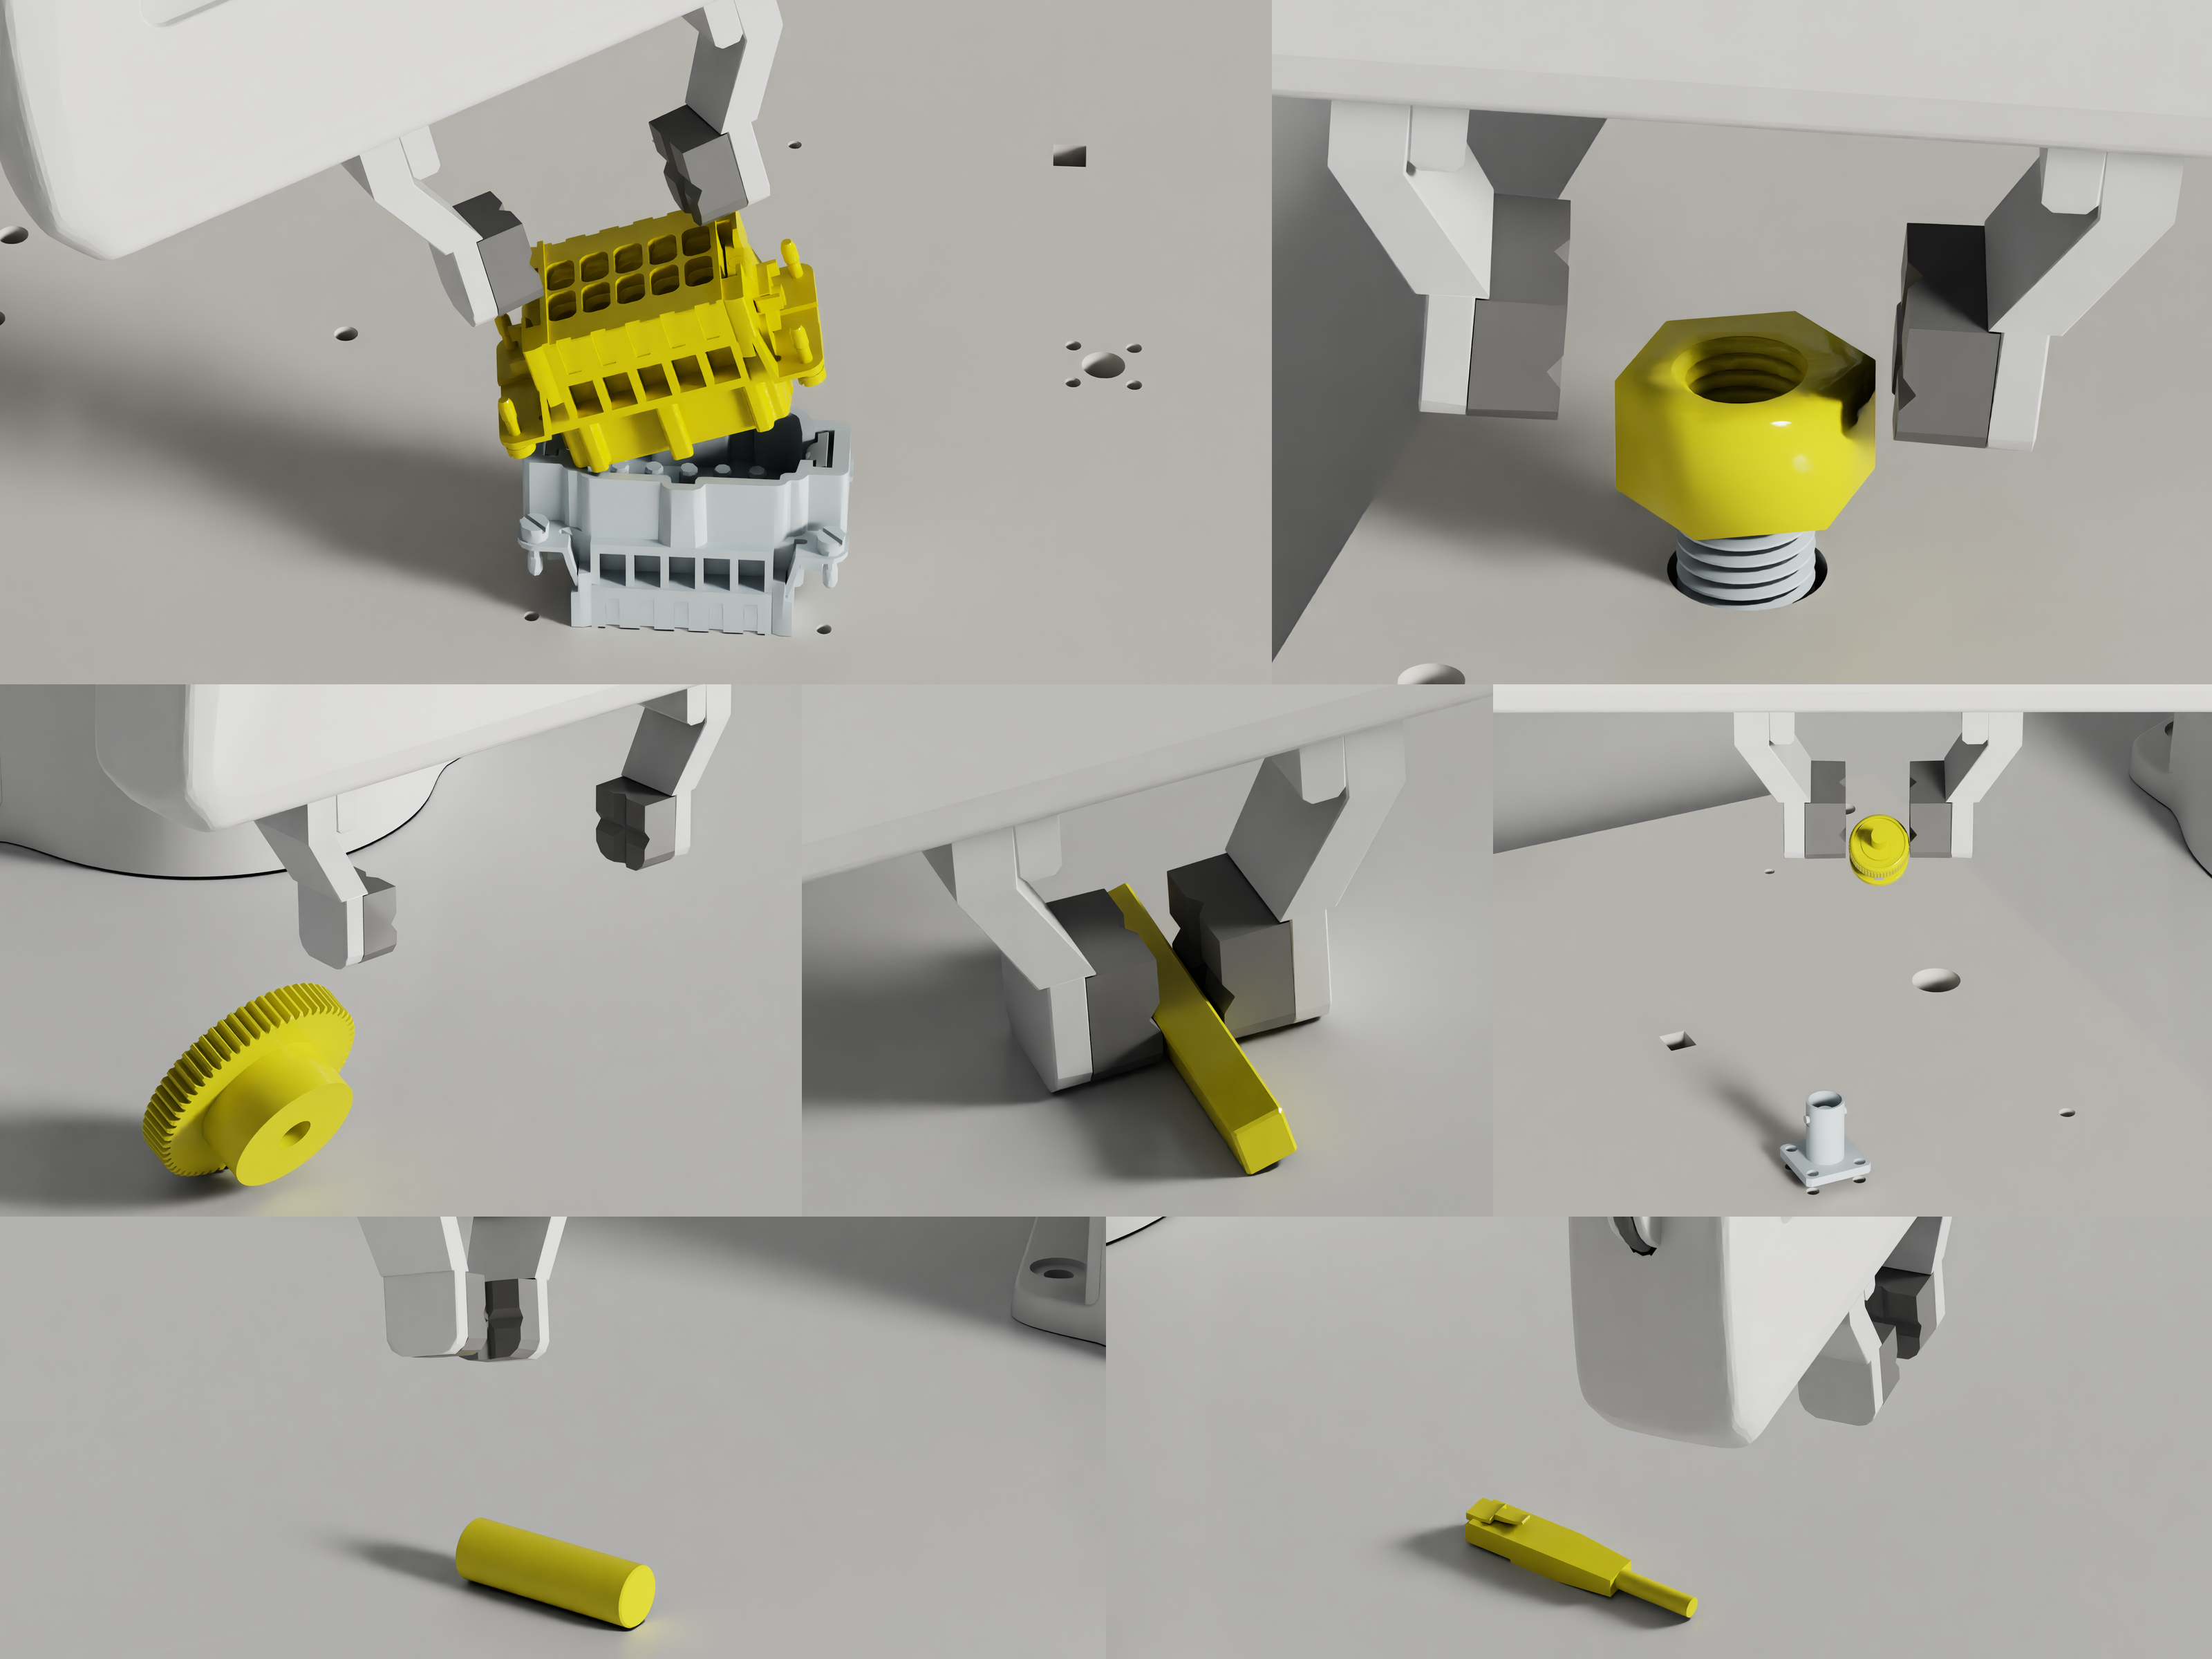
\includegraphics[width=\columnwidth]{figures/method/reset_coverage.png}
    \caption{\textbf{Diverse assembly reset states.} Examples of resets across
    tasks, ranging from random object poses to in-hand grasps and partial
    assemblies.}
    \label{fig:reset-coverage}
\end{figure}



Let $\hat{p}_i$ be the empirical success rate over the most recent $L$ episodes
initialized from entry $(e_i,\bar{s}_i)$. Under beta sampling, entry $i$ is
selected with probability $q_i$:
\begin{equation}
    q_i\propto \varepsilon_q+
    \sqrt{\hat{p}_i(1-\hat{p}_i)},\qquad i=1,\ldots,M,
    \label{eq:beta-sampling}
\end{equation}
normalized over the entire bank. Sampling $i\sim\operatorname{Cat}(\mathbf q)$
selects an assembly--reset pair with $\rho(e_i,\bar{s}_i)=q_i$.
The kernel favors intermediate success rates, while $\varepsilon_q>0$
keeps every entry sampleable. Each episode's outcome updates $\hat{p}_i$
for its sampled entry.
The uniform ablation sets $q_i=1/M$; the bank, policy, reward, and
optimizer remain unchanged.
Algorithm~\ref{alg:training} summarizes training.



\subsection{Binary Full-Assembly Objective}

Across geometries, the assembly objective is the same: complete the assembly.
For each instance, an assembly-relative coordinate $\Phi_e(\alpha)$,
$\alpha\in[0,1]$, parameterizes the part in the mating frame, with
$\Phi_e(1)$ denoting its fully assembled pose. Let $d_{\mathrm{asm}}^e(s)$ be
the distance between the part's current relative pose and $\Phi_e(1)$.
For a single-pair episode, the binary task reward is
\begin{equation}
    r_t^{\mathrm{succ}}
    =
    \begin{cases}
        1, & d_{\mathrm{asm}}^e(s_{t+1})<\epsilon,\\
        0, & \text{otherwise}.
    \end{cases}
    \label{eq:sparse-reward}
\end{equation}
where $\epsilon=0.001\,\mathrm{m}$.
The success reward is issued once, and the episode terminates.
Intermediate progress receives no task reward.
We supplement the binary task reward with a control cost to discourage
large action magnitudes, rapid joint motion, and excessive torque.
This regularization biases learning toward smoother, lower-effort behaviors that are more compatible with safe deployment on physical robots, without providing information about assembly progress.
\begin{equation}
    r_t = \underbrace{r_t^{\mathrm{succ}}}_{\text{binary task reward}} - \underbrace{c\left(\lVert a_t\rVert_2^2 + \lVert \dot{q}_t\rVert_2^2 + \lVert \tau_t\rVert_2^2\right)}_{\text{control cost}}, \quad c \geq 0.
    \label{eq:full-reward}
\end{equation}
Here, $a_t$, $\dot{q}_t$, and $\tau_t$ are the action, robot joint velocity, and
applied joint torque. The control penalties are evaluated at every step,
with a single coefficient $c$ fixed across tasks. They do not measure
assembly progress; the binary task reward specifies successful completion.
Episodes end on assembly success, at horizon $T$, or when an arm joint
exceeds its hardware velocity or torque limit. %
In multi-pair episodes, the success reward remains zero until every active pair is
assembled, with no prescribed pair order or intermediate completion
reward.



\begin{figure*}[t]
    \centering
    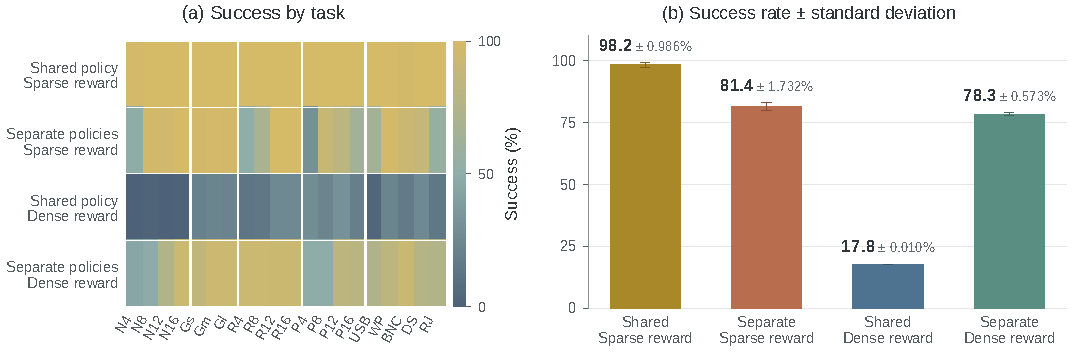
\includegraphics[width=\textwidth]{figures/results/heterogeneity.pdf}
    \caption{
    \textbf{Training across heterogeneous assembly pairs substantially improves learning from a sparse binary task reward.}
    At 64K environments across 25k iterations: (a) compares 20-task success rates for
    one shared policy versus 20 separately trained policies. The shared policy (first row)
    achieved above 98\% success rate across all tasks, including three precision assemblies that corresponding specialists rarely solve. Dense shaping does not exhibit the same benefit.
    Panel (b) shows overall success, note that the separate-policy success rate is average across all 20 per-task policies;
    \textit{Asset notation:} N, G, R, and P denote nuts, gears, rods, and pegs, respectively; numeric
    suffixes indicate nominal diameters in millimeters, while s, m,
    and l indicate gear size.
    "Sparse reward" denotes Eq. (6); "dense reward" additionally includes the shaping terms in Eq. (7).
    }
    \label{fig:heterogeneity-ablation}
\end{figure*}

\begin{figure}[!tb]
    \centering
    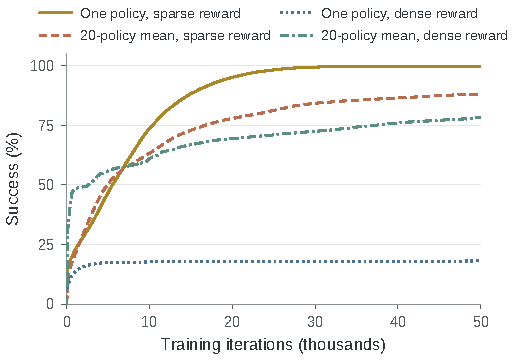
\includegraphics[width=\columnwidth]{figures/results/heterogeneity_dynamics.pdf}
    \caption{\textbf{Joint sparse training converges faster than separate
    policies.} Curves compare one shared policy trained on all 20 tasks with
    the mean of 20 policies trained separately, one per task.}
    \label{fig:heterogeneity-dynamics}
\end{figure}

\begin{figure}[!tb]
    \centering
    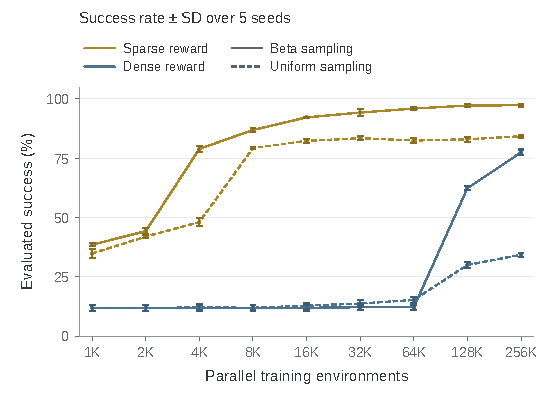
\includegraphics[width=\columnwidth]{figures/results/scaling.pdf}
    \caption{
    \textbf{Sparse task rewards benefit strongly from parallel experience.}
    Mean success $\pm$ standard deviation over 5 evaluation seeds for 
    25k-iteration checkpoints, with 32 trials per task per seed across 20
    assemblies. Color denotes reward; solid and
    dashed lines denote beta and uniform training-reset sampling.}
    \label{fig:parallel-scaling}
\end{figure}


\begin{figure*}[!tb]
    \centering
    \setlength{\tabcolsep}{2pt}
    \begin{tabular}{@{}cc@{}}
        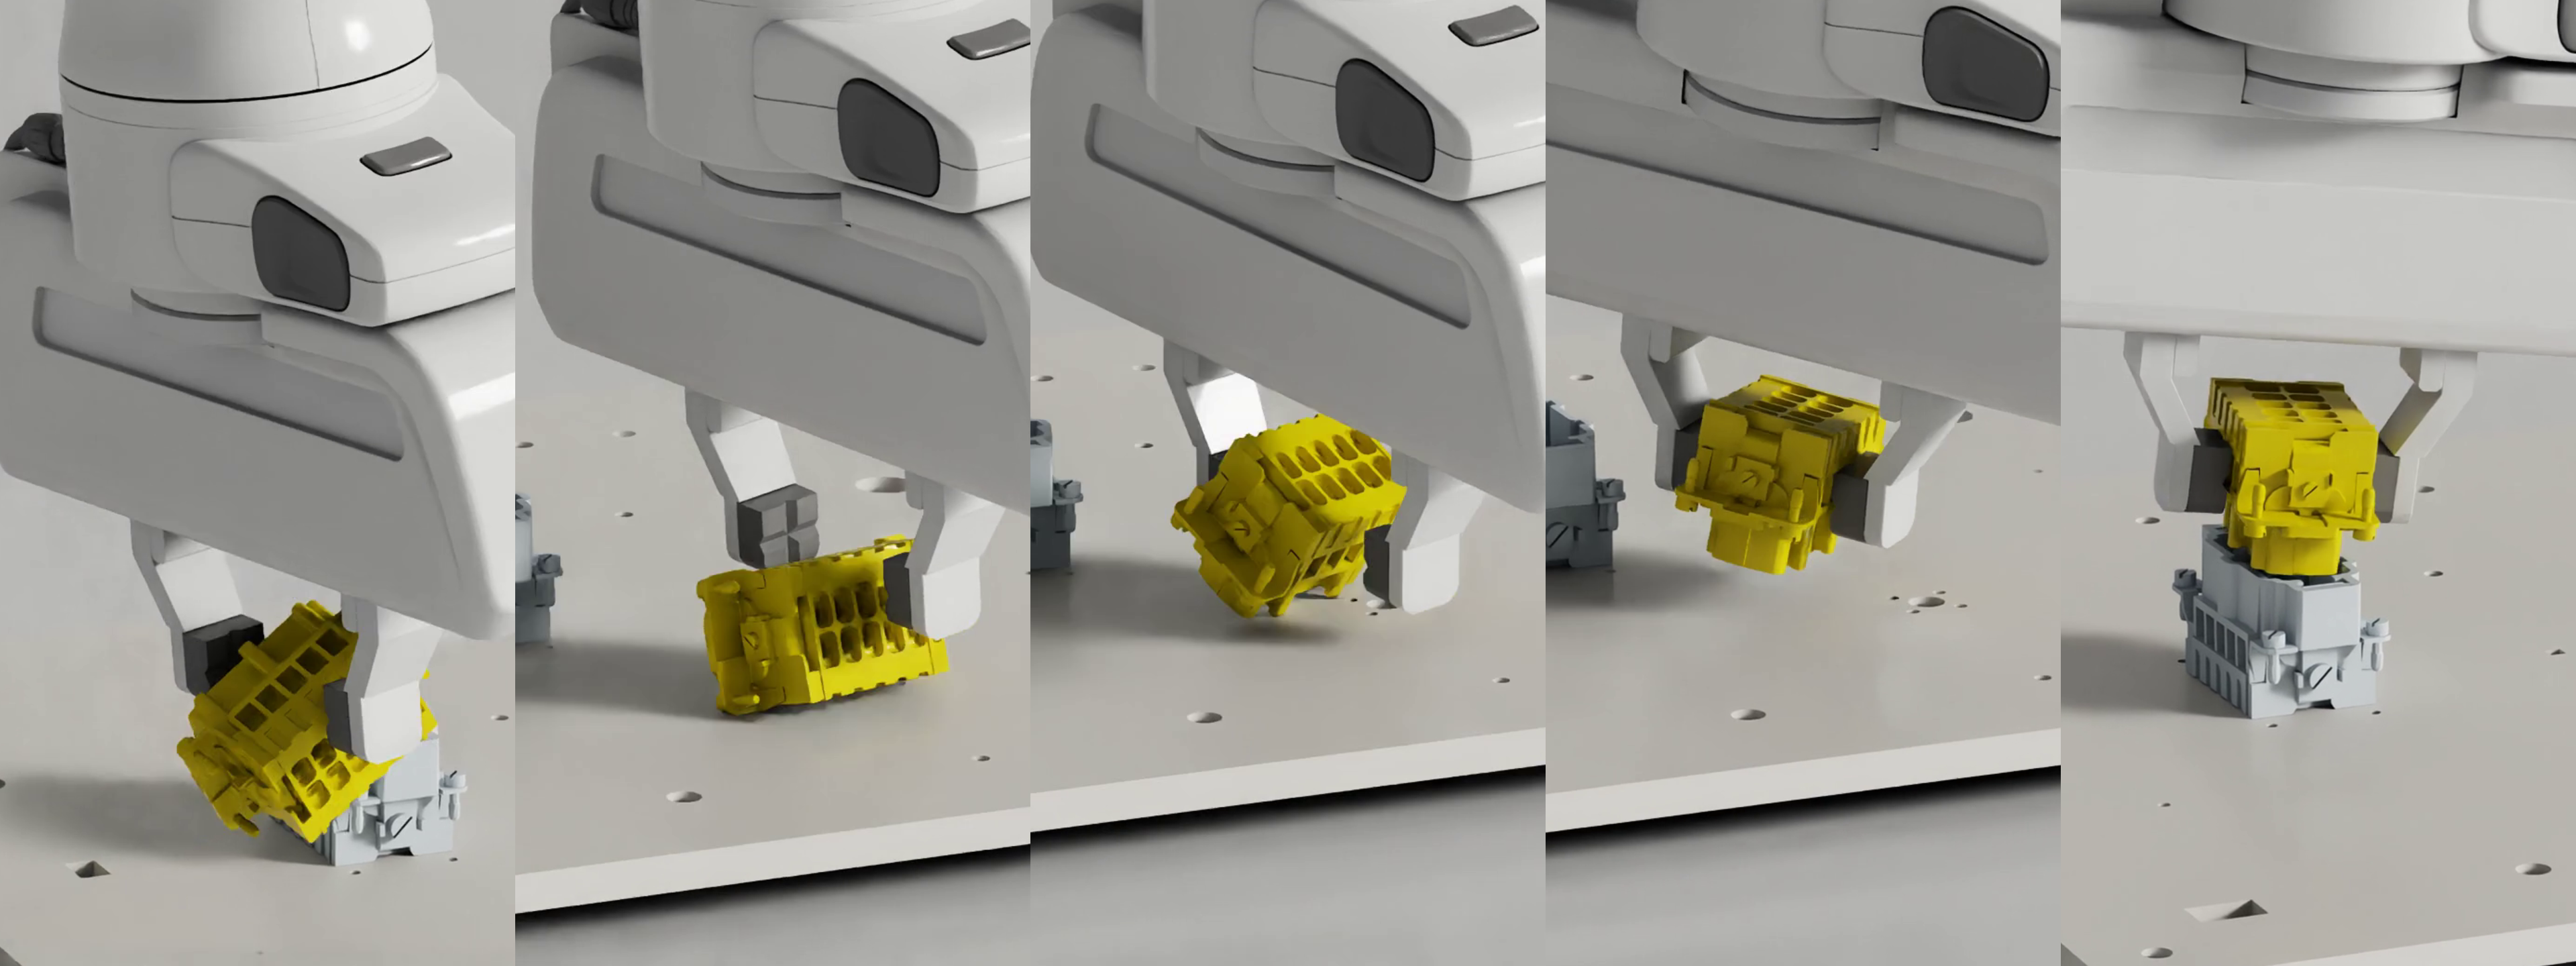
\includegraphics[width=0.485\textwidth,trim=0 36 0 144,clip]{figures/qualitative/waterproof_strategy.png} &
        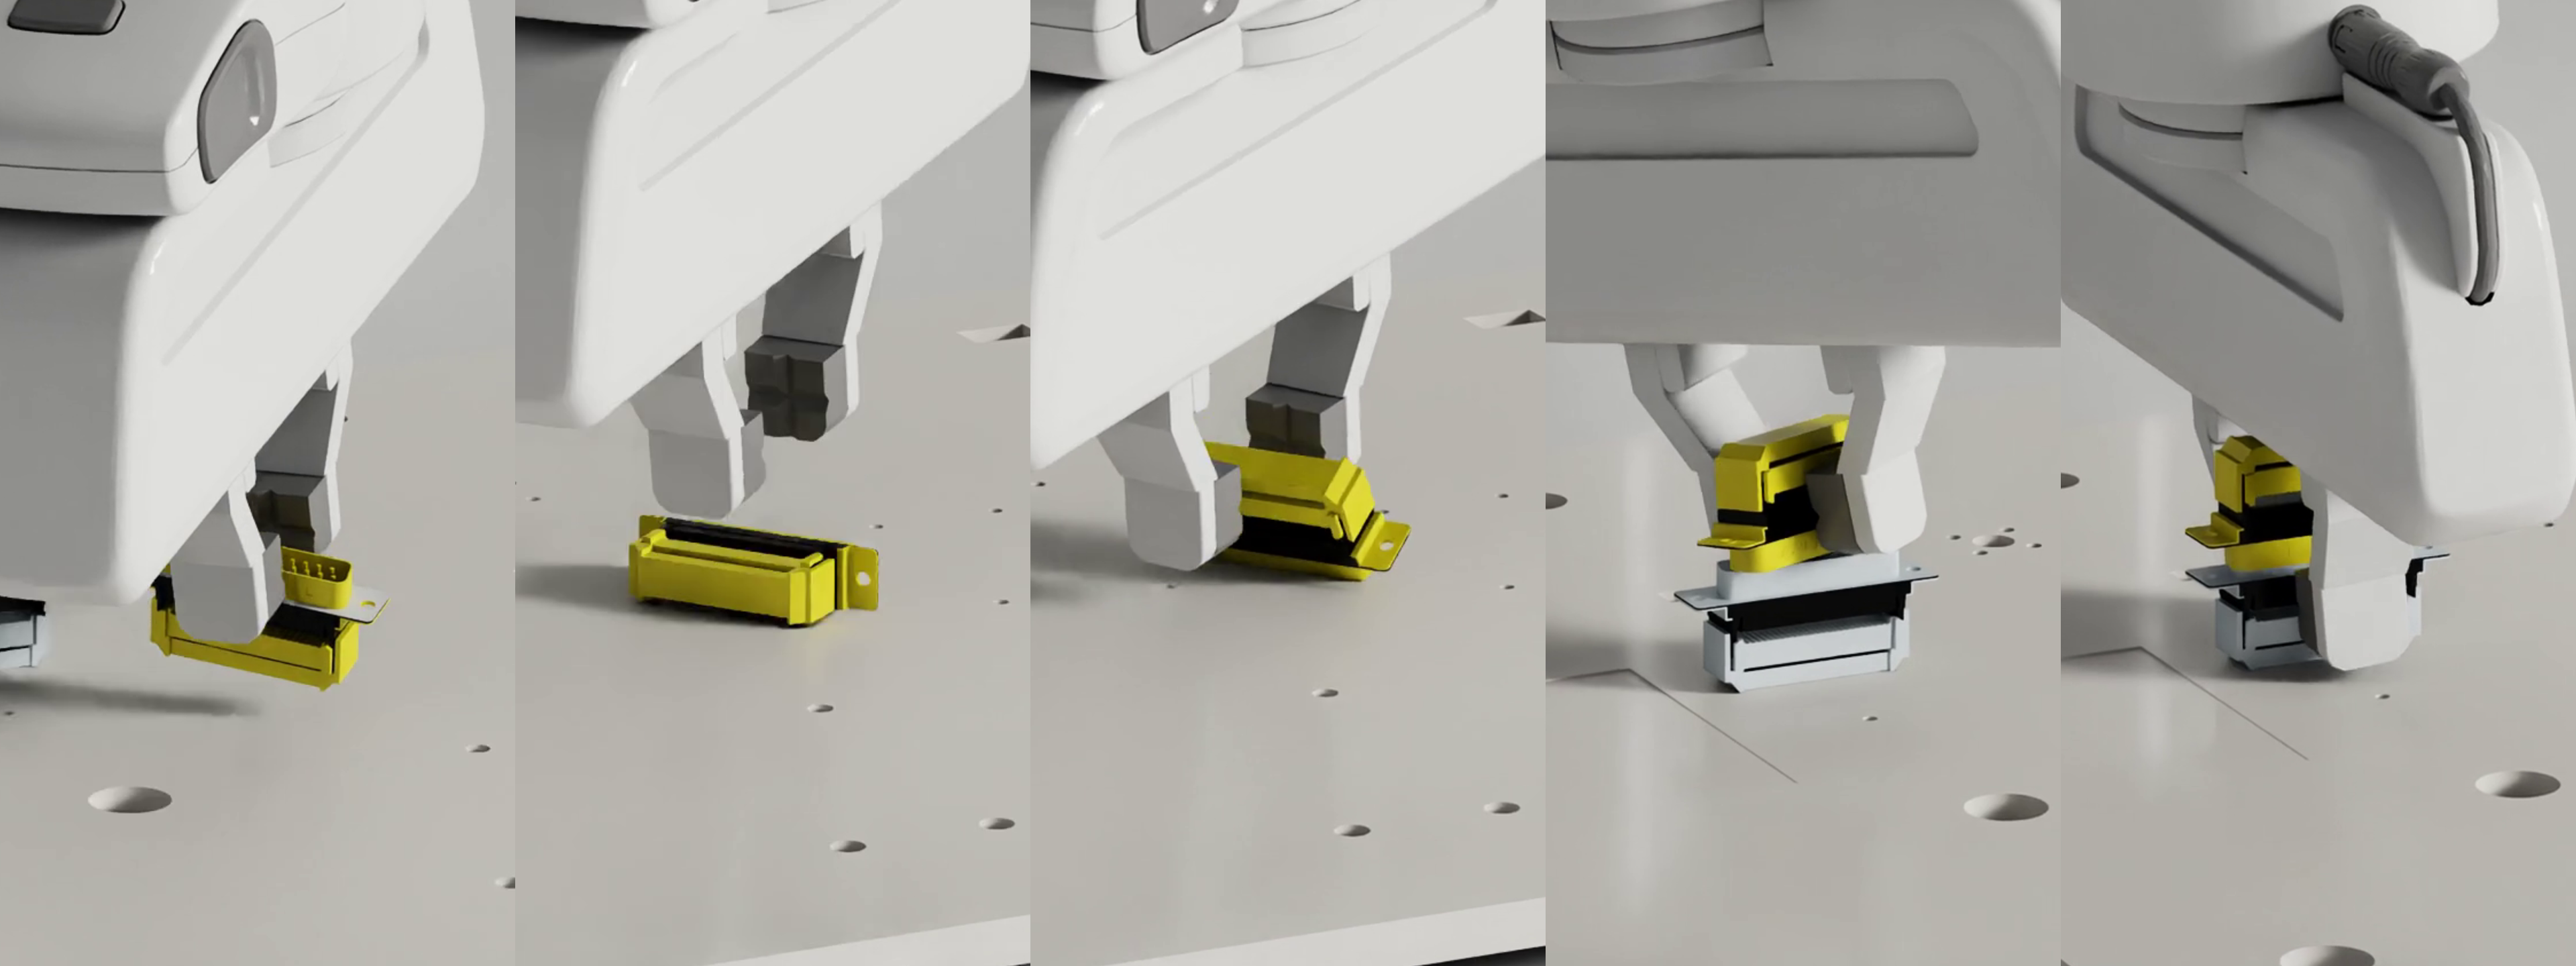
\includegraphics[width=0.485\textwidth,trim=0 36 0 144,clip]{figures/qualitative/dsub_strategy.png} \\
        \footnotesize\sffamily\textbf{(a)} Board-assisted reorientation(waterproof) &
        \footnotesize\sffamily\textbf{(b)} Release-and-regrasp for alignment(d-sub) \\[2pt]
        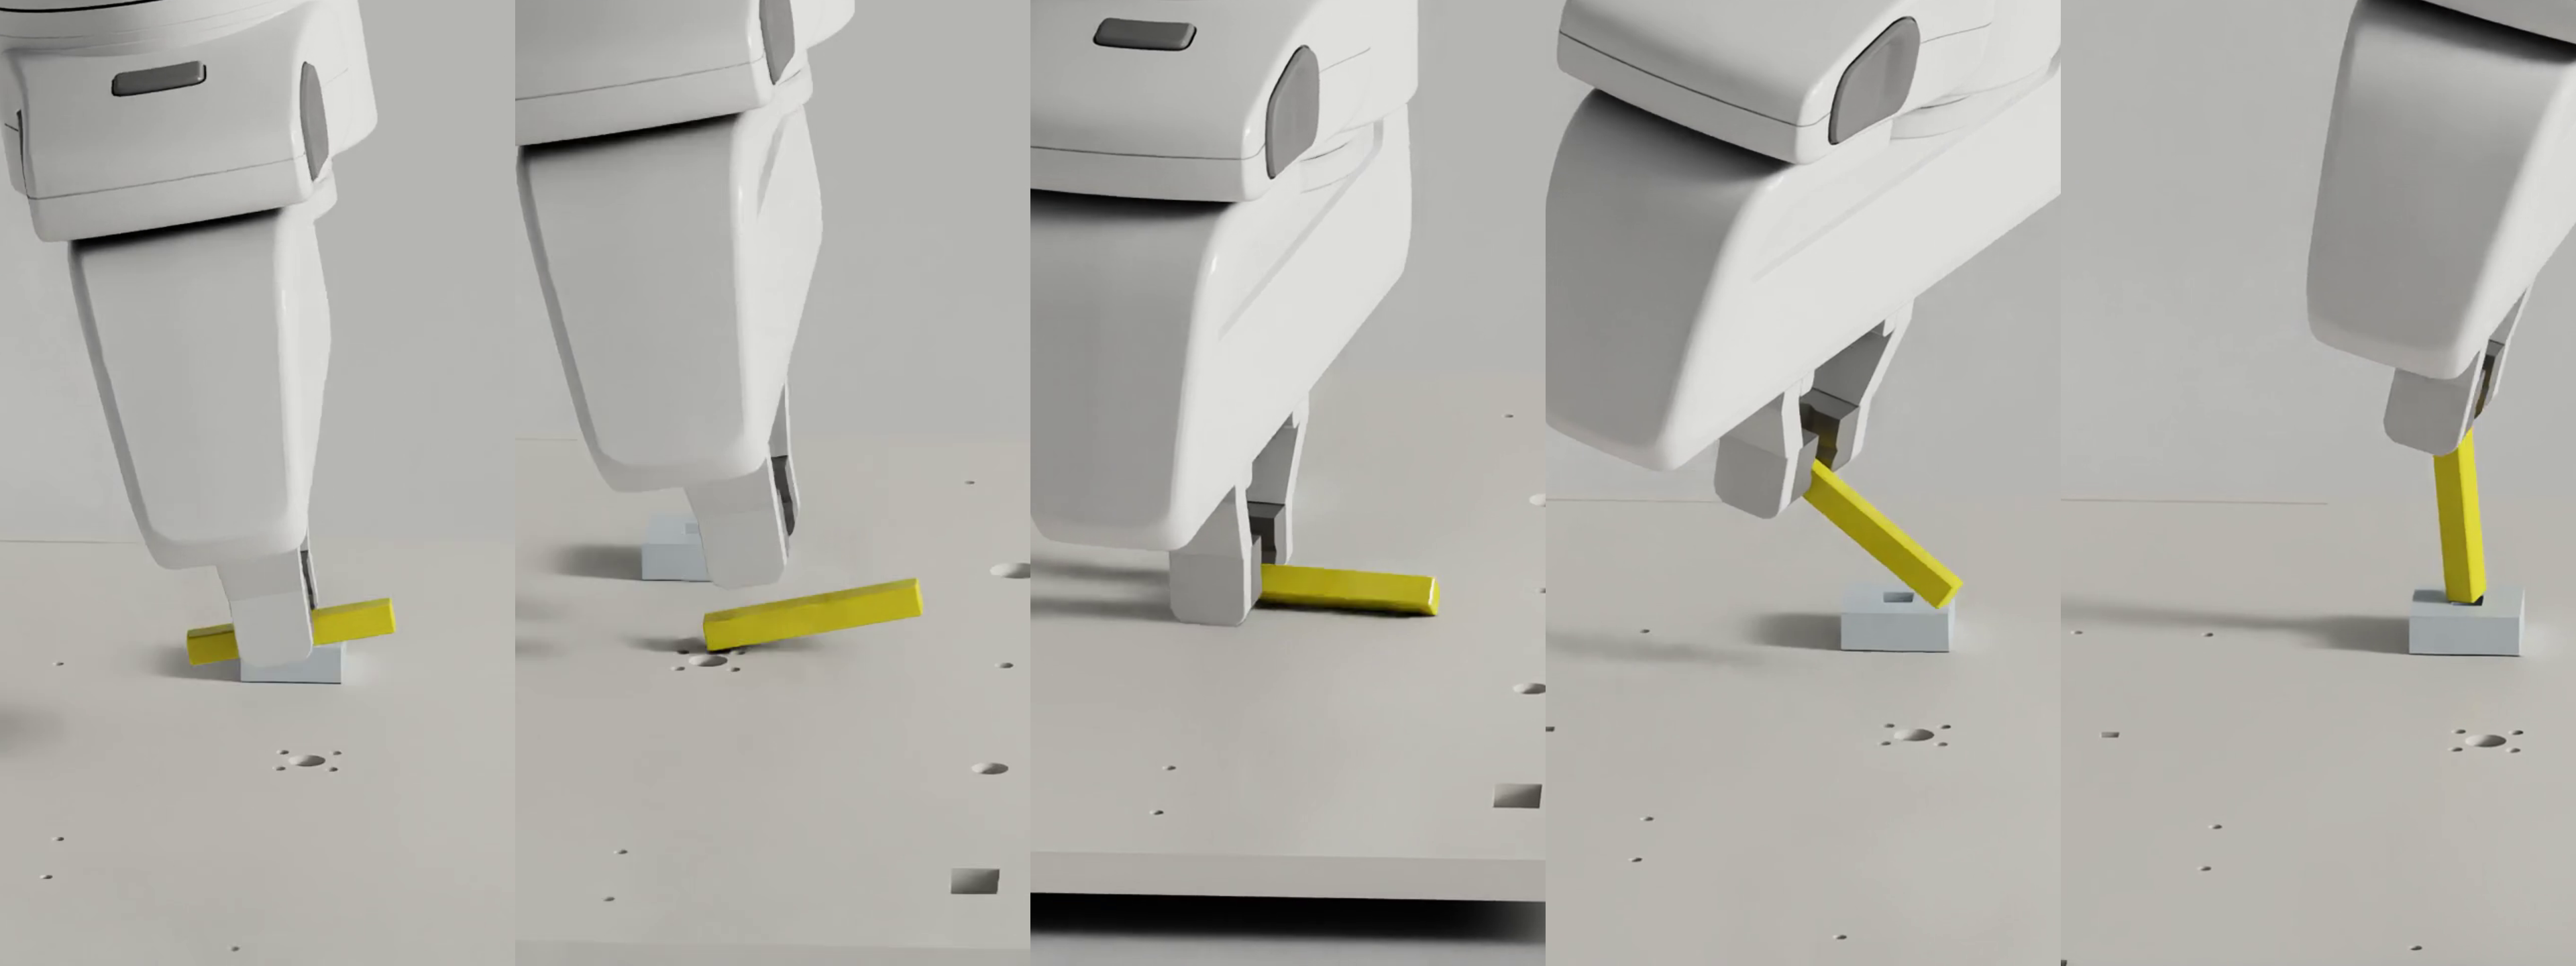
\includegraphics[width=0.485\textwidth,trim=0 36 0 144,clip]{figures/qualitative/peg_insert_8mm_strategy.png} &
        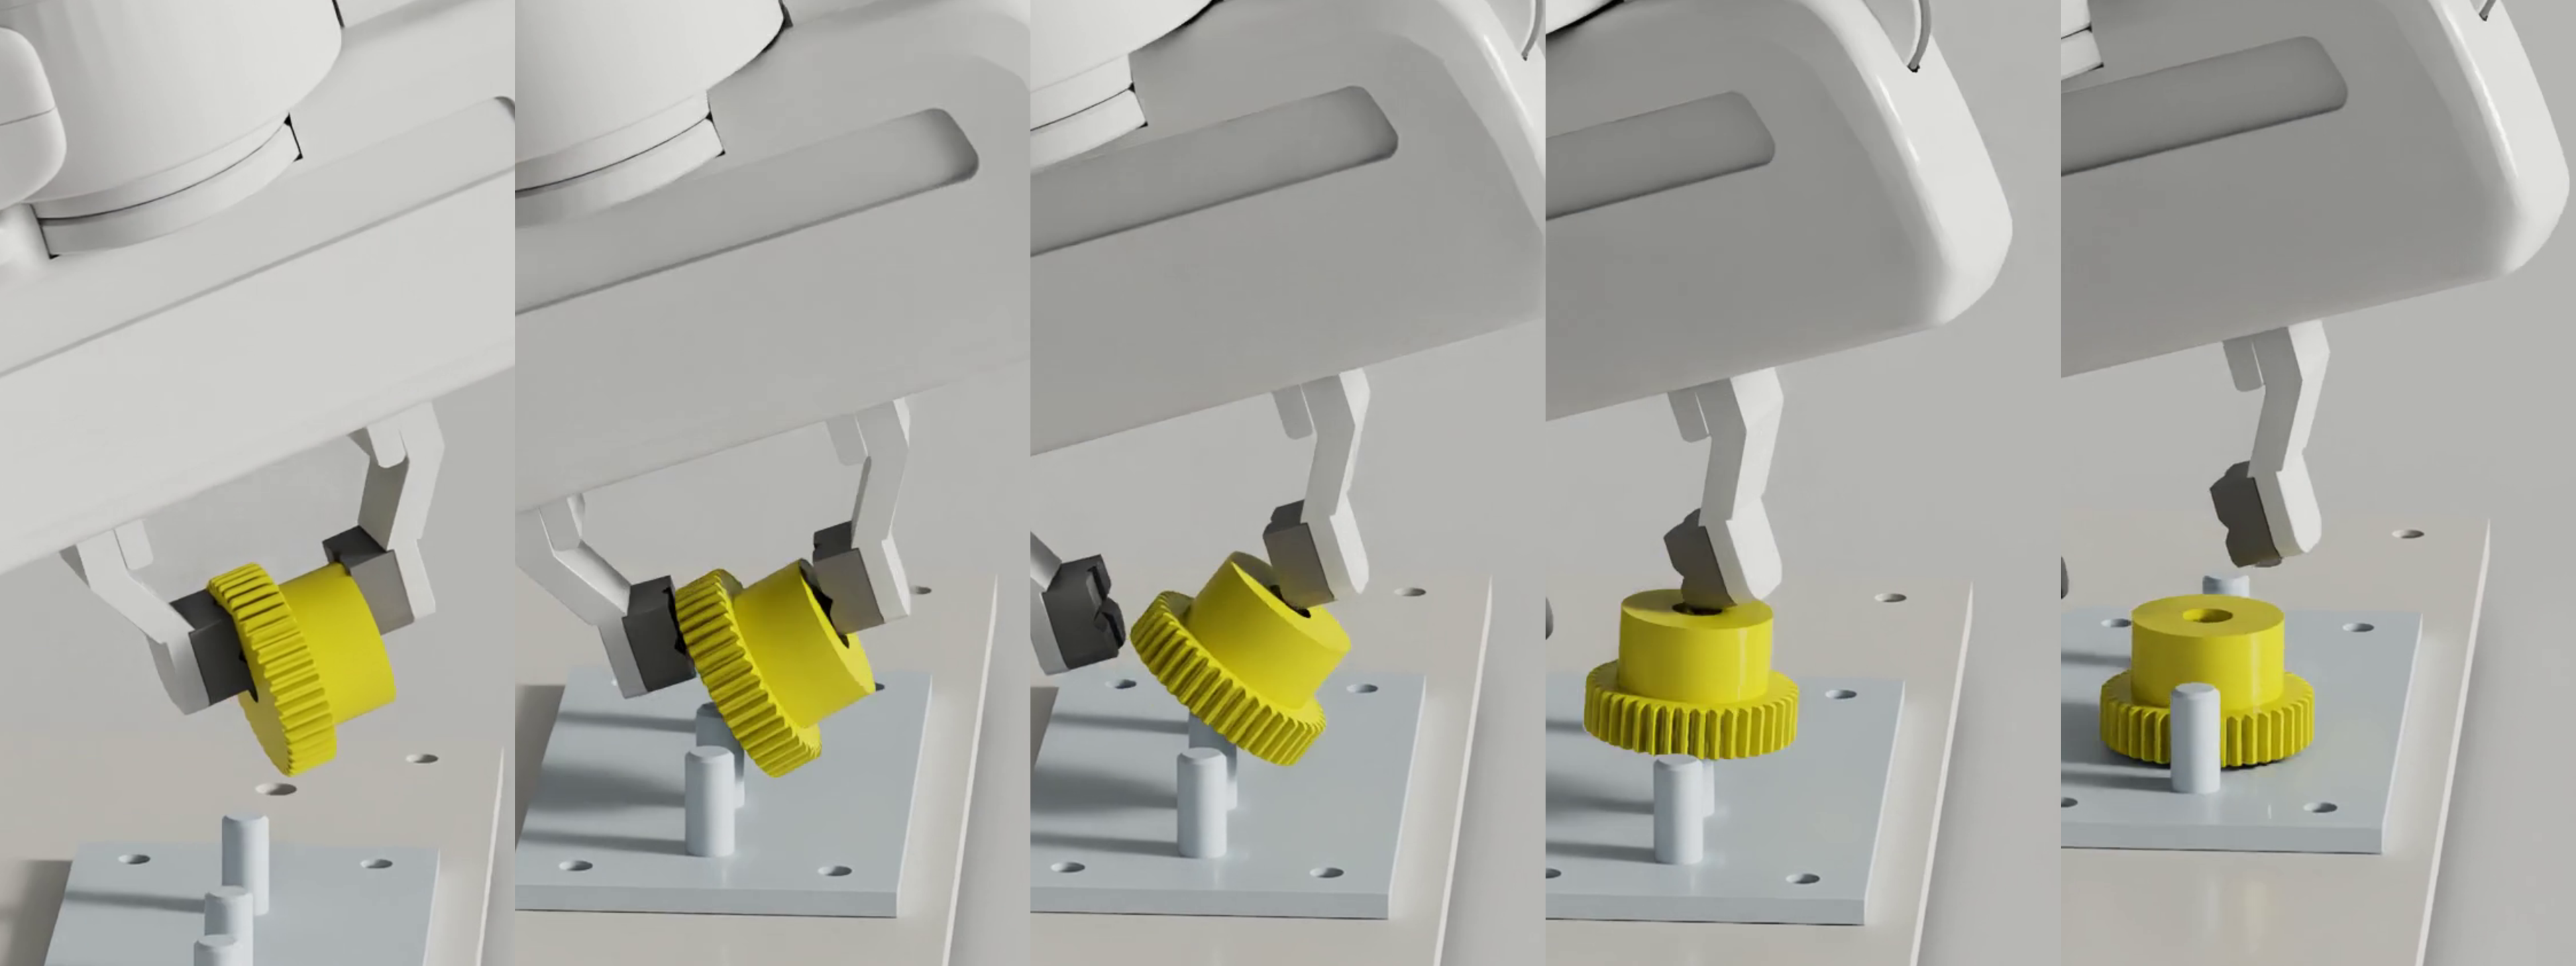
\includegraphics[width=0.485\textwidth,trim=0 36 0 144,clip]{figures/qualitative/gear_mesh_medium_strategy.png} \\
        \footnotesize\sffamily\textbf{(c)} Center-to-tip grasp transfer(peg 8mm) &
        \footnotesize\sffamily\textbf{(d)} Side-caging for gear placement(medium gear) \\[2pt]
        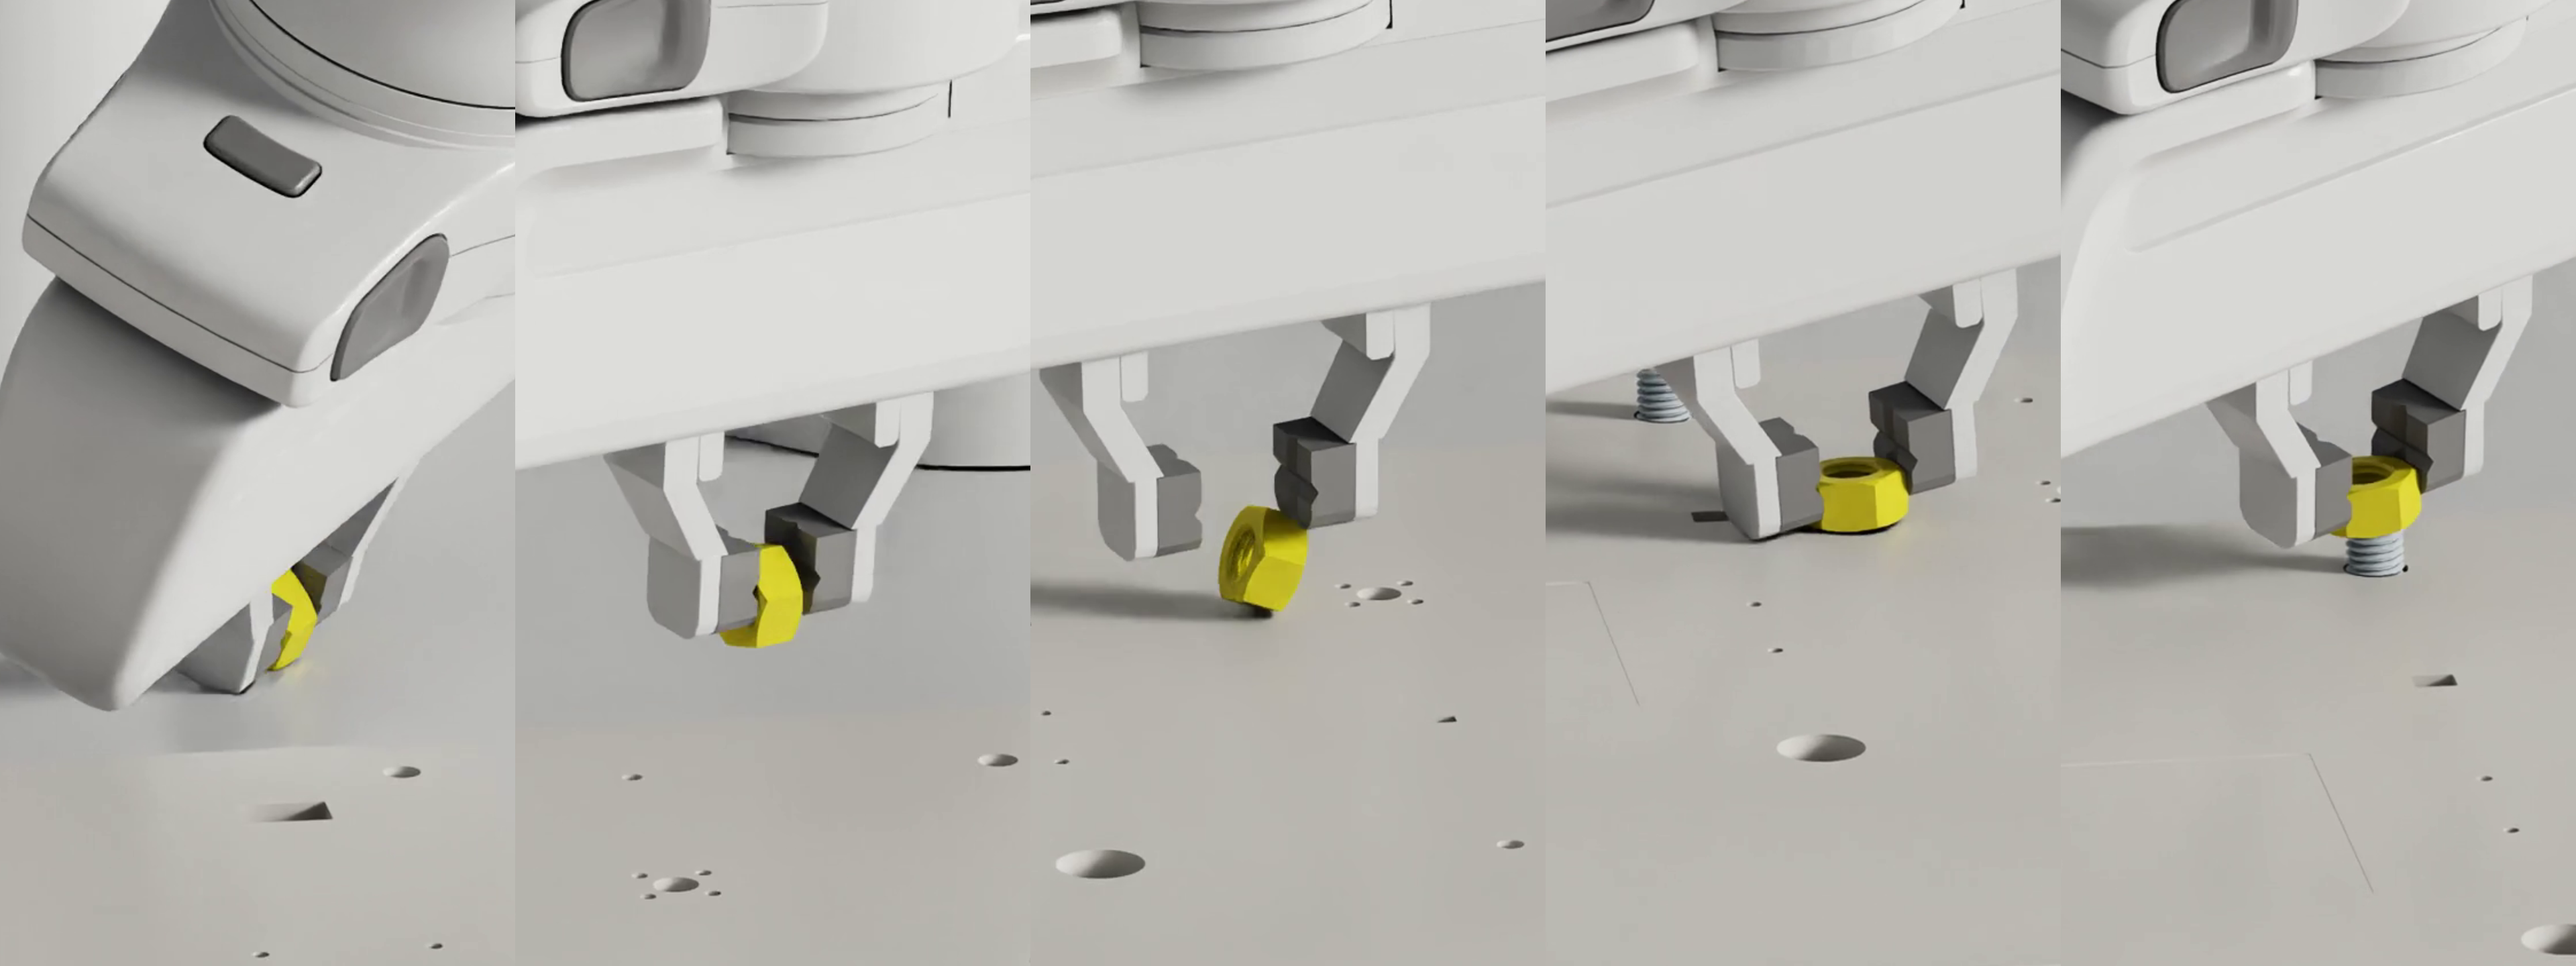
\includegraphics[width=0.485\textwidth,trim=0 36 0 144,clip]{figures/qualitative/nut_thread_m12_strategy.png} &
        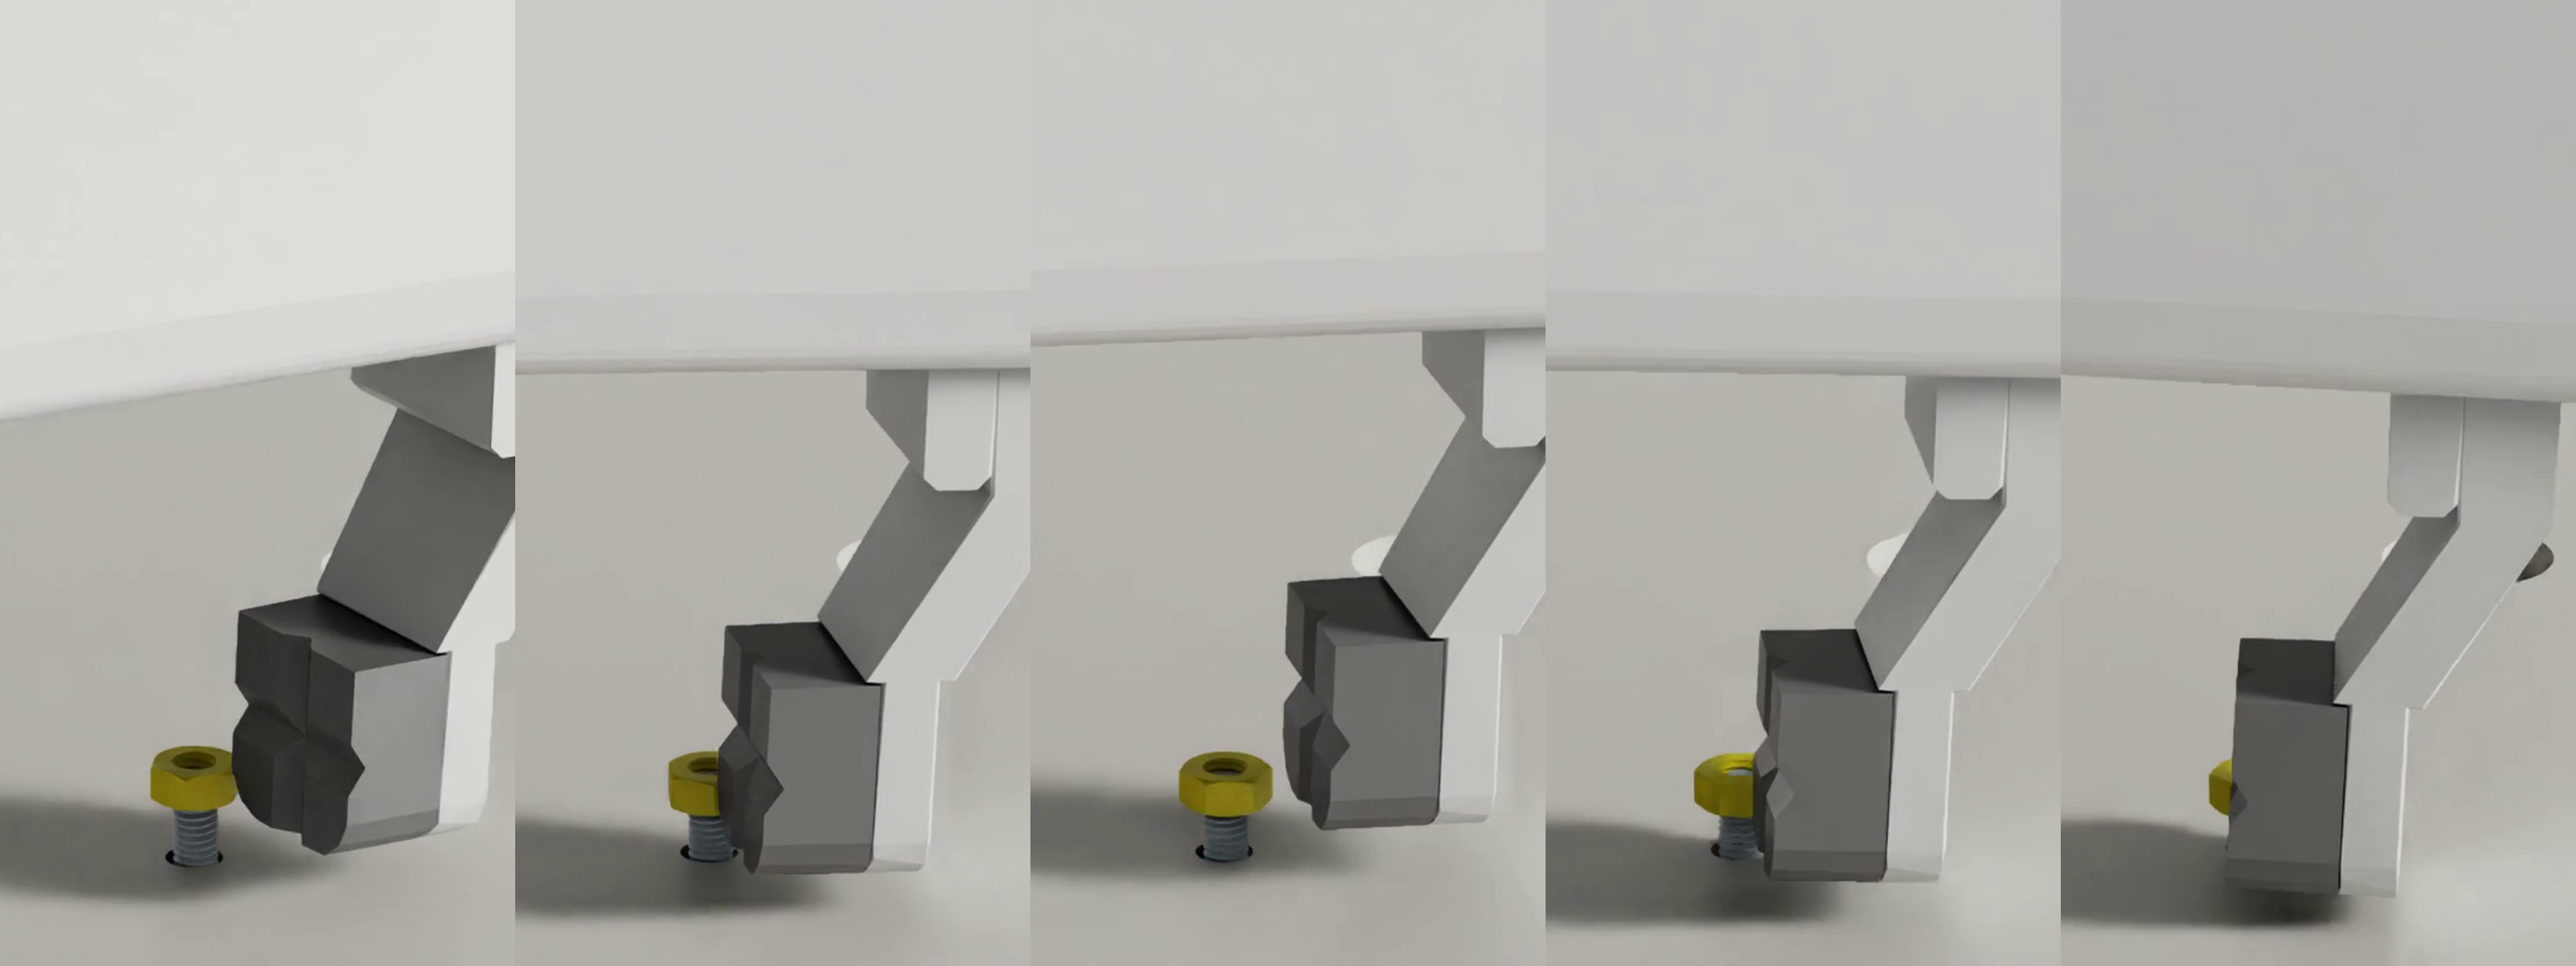
\includegraphics[width=0.485\textwidth,trim=0 0 0 180,clip]{figures/qualitative/nut_thread_m4_strategy.png} \\
        \footnotesize\sffamily\textbf{(e)} Edge-to-flat nut reorientation(nut m12) &
        \footnotesize\sffamily\textbf{(f)} One-sided tapping for threading(nut m4) \\[2pt]
        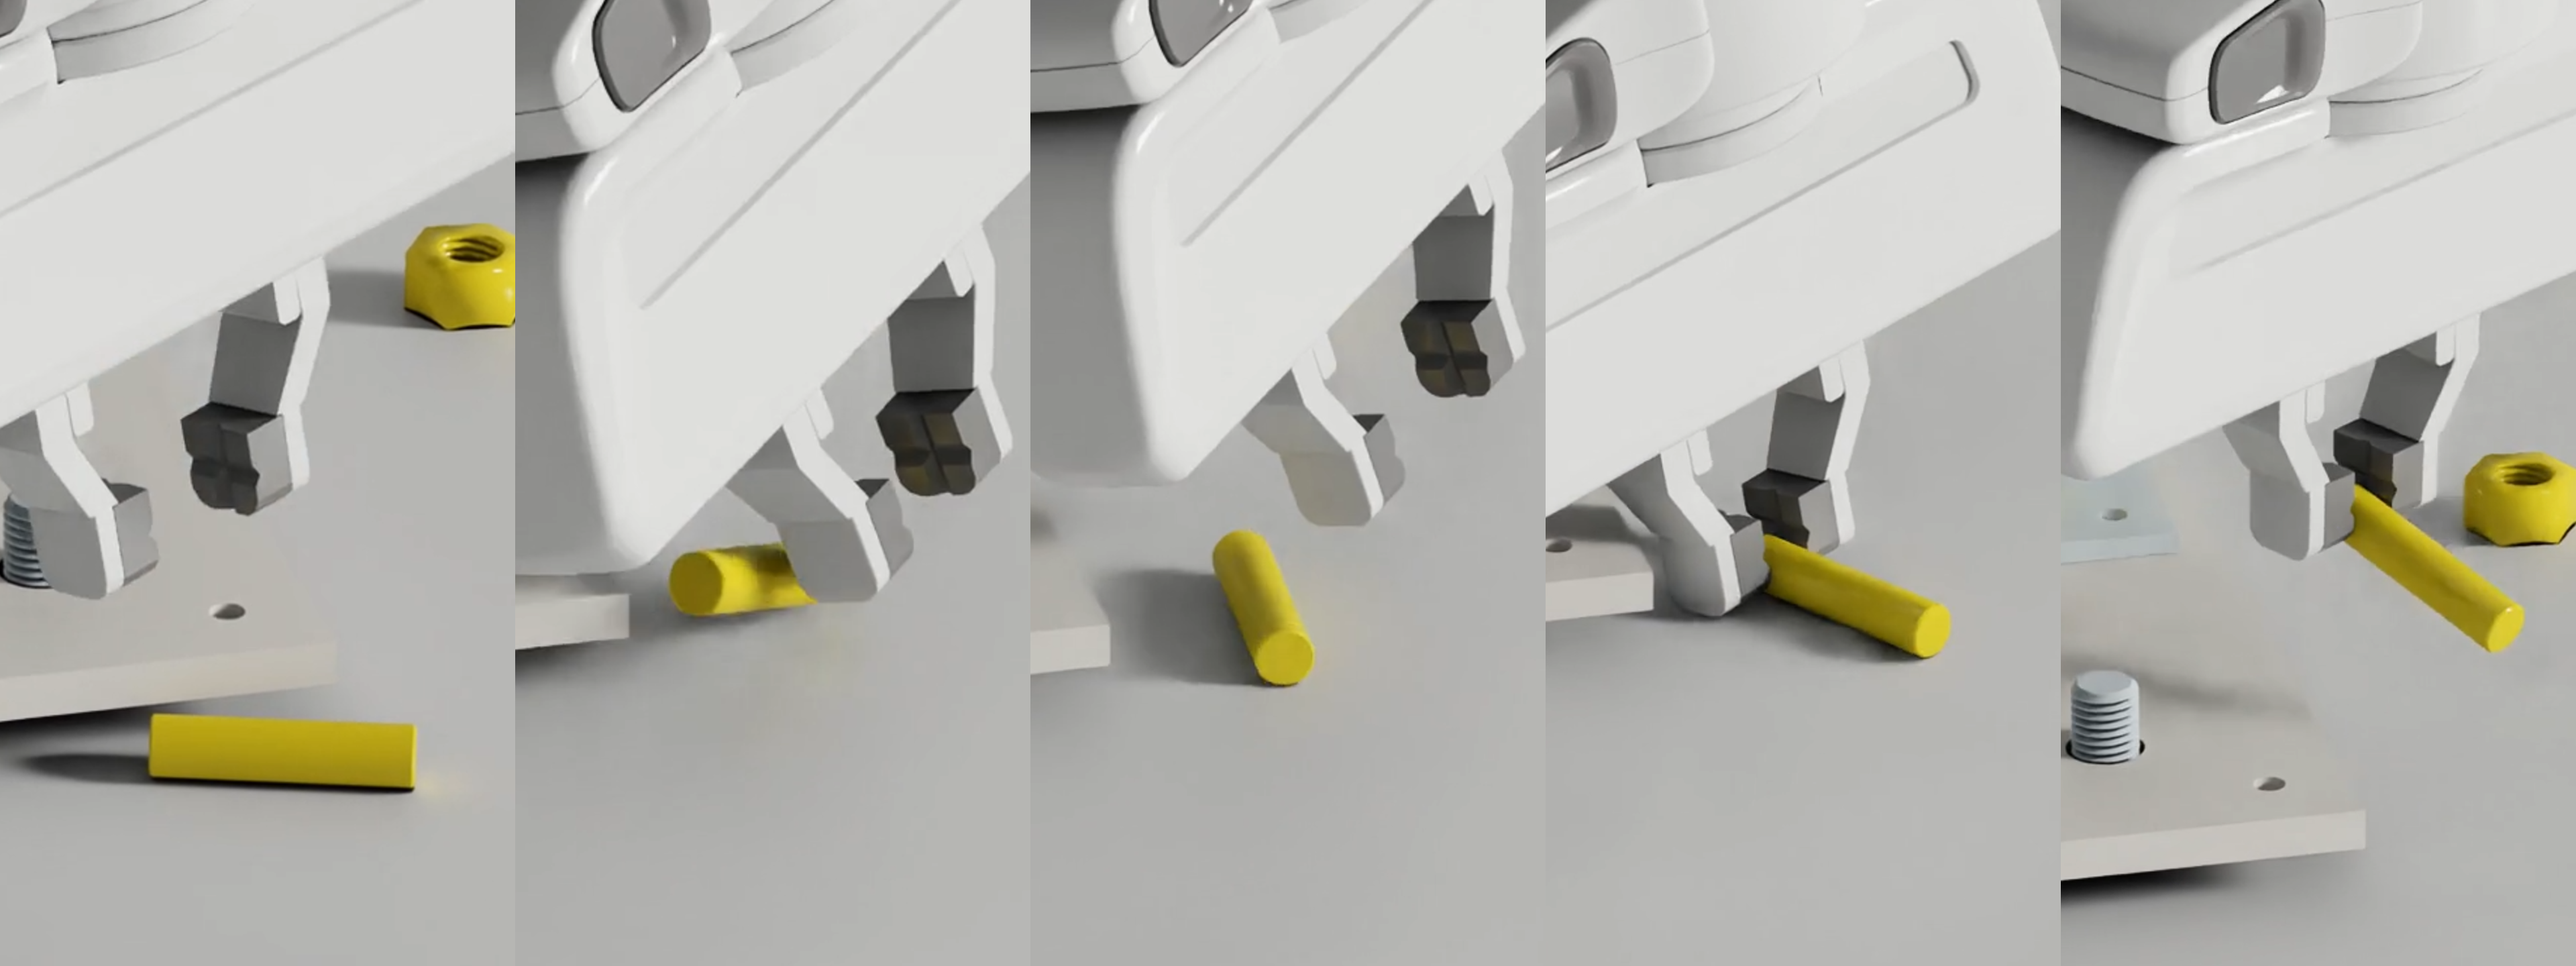
\includegraphics[width=0.485\textwidth,trim=0 36 0 144,clip]{figures/qualitative/shoveling_rod_8mm.png} &
        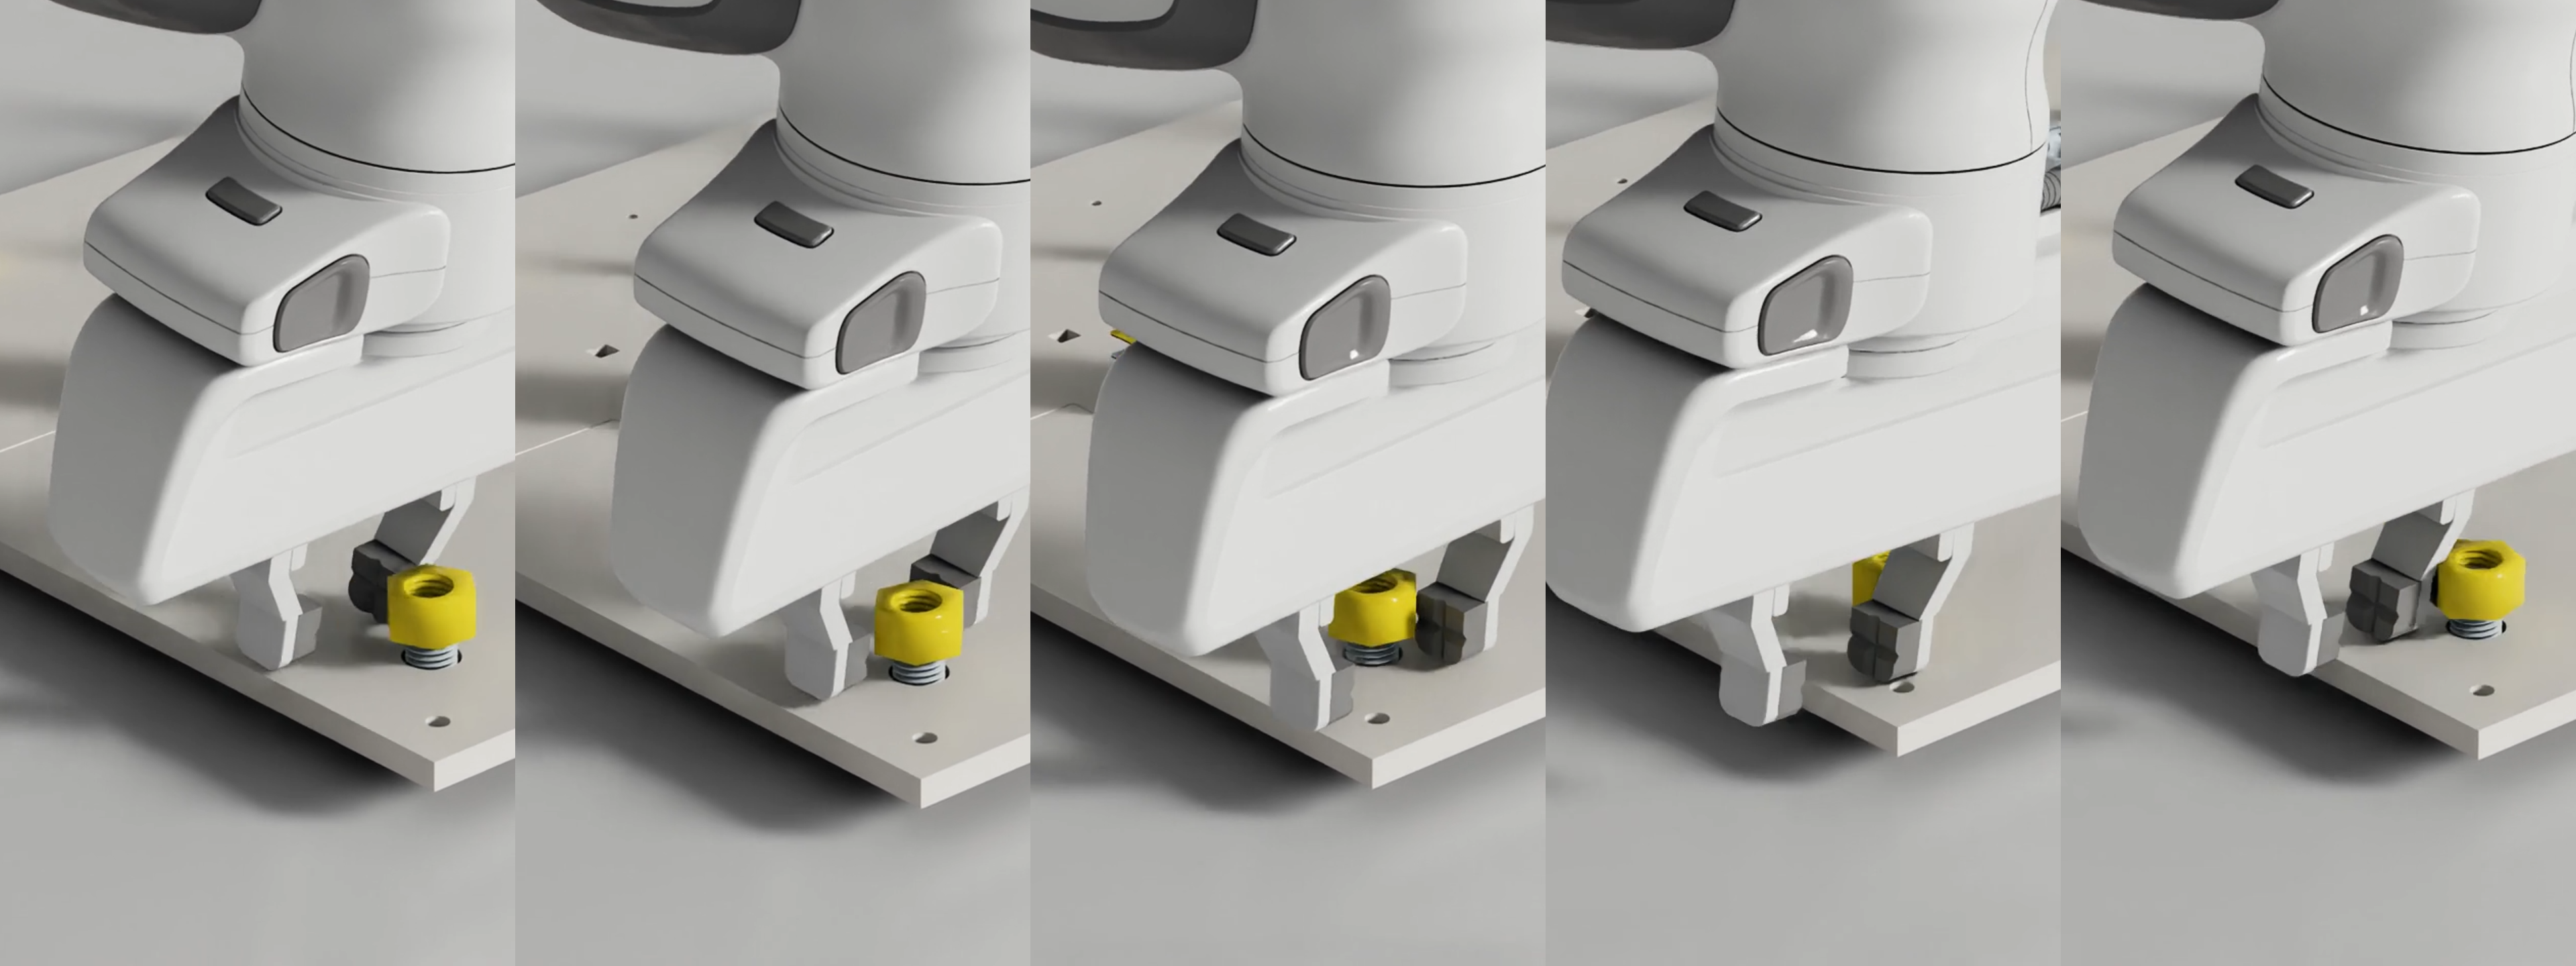
\includegraphics[width=0.485\textwidth,trim=0 36 0 144,clip]{figures/qualitative/full_circle_threading_m16.png} \\
        \footnotesize\sffamily\textbf{(g)} Shoveling to a better pickup position(rod 8mm) &
        \footnotesize\sffamily\textbf{(h)} Full-circle nut threading(nut m16)
    \end{tabular}
    \caption{\textbf{One shared policy discovers diverse contact strategies
    from a sparse binary task reward.} Each panel proceeds from left to right.
    (a) Waterproof connector: board contact helps reorient the part before insertion.
    (b) D-sub connector: the part is set down and regrasped for alignment with its socket.
    (c) 8 mm peg: the part is dropped from a center grasp and regrasped near one end,
    leaving its remaining length free for insertion.
    (d) Medium gear: the part pivots from a side grasp into a horizontal pose over its
    mounting post. (e) M12 nut: the nut is rolled from its edge onto a flat face before
    placement on the bolt. (f) M4 nut: repeated one-sided taps advance the nut along
    the thread. (g) 8 mm rod: the fingertip shovels the rod to a position where it is
    easier to lift. (h) M16 nut: the gripper moves around the nut, using fingertip
    contact to turn it along the bolt.}
    \label{fig:emergent-assembly-strategies}
\end{figure*}

\begin{figure*}[!tb]
    \centering
    \begin{tabular}{@{}c@{}}
        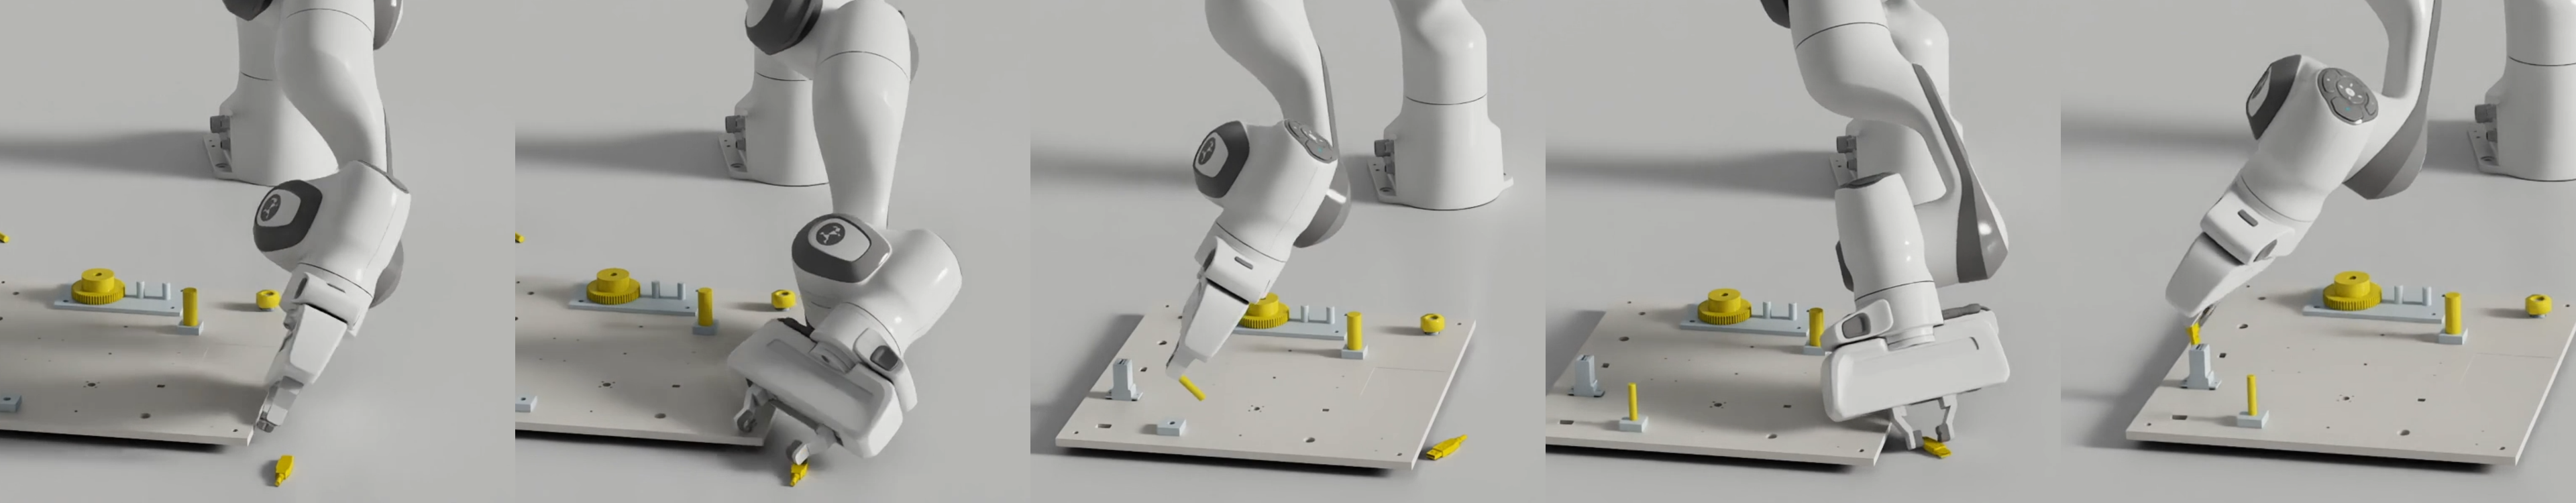
\includegraphics[width=\textwidth]{figures/qualitative/bring_close_deferred_assembly.png} \\
        \footnotesize\sffamily\textbf{(a)} Bring USB-A closer, assemble the 8 mm rod, then return \\[4pt]
        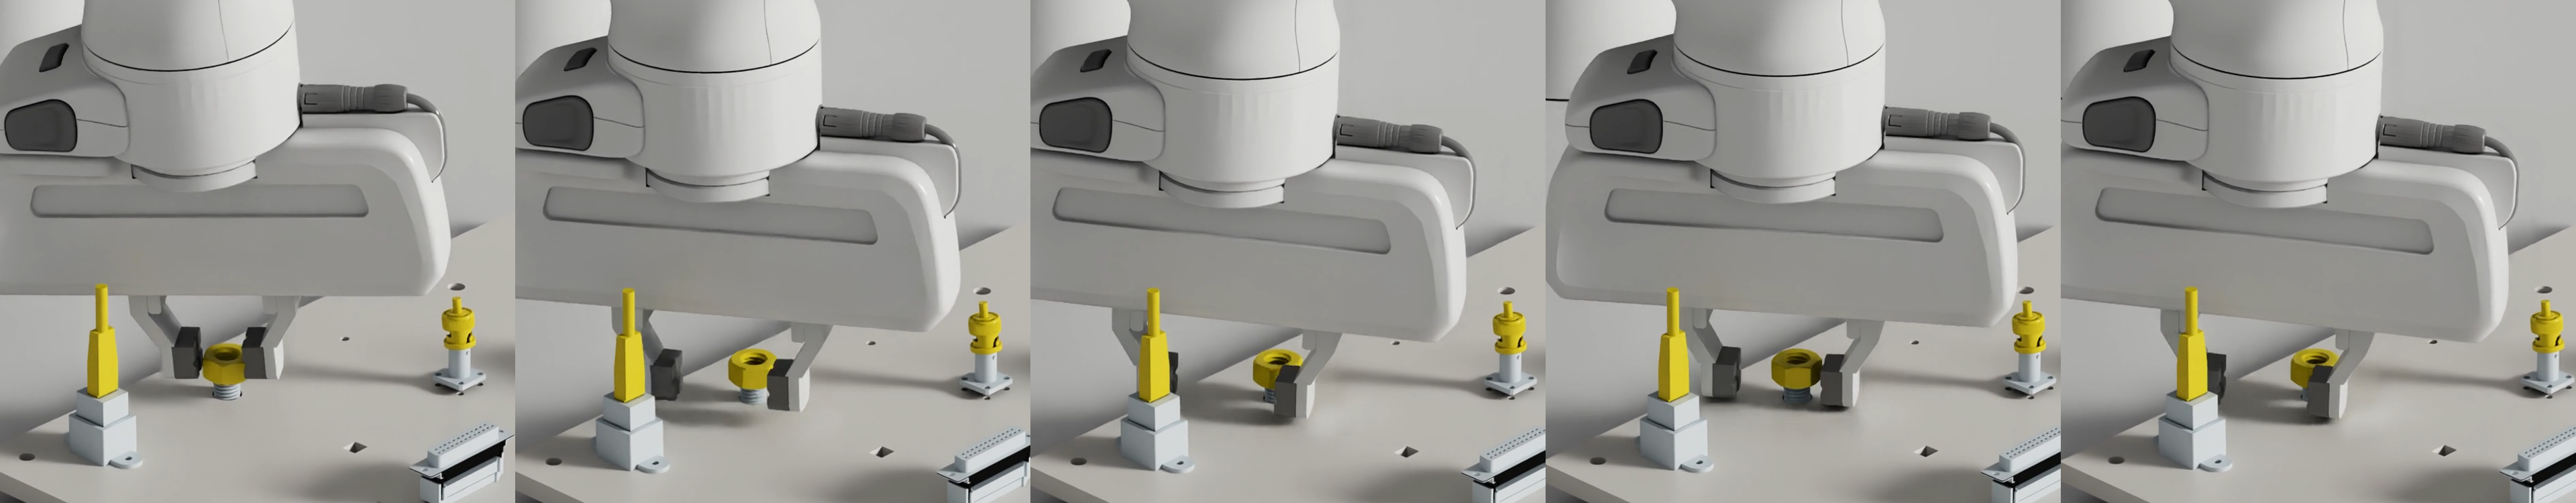
\includegraphics[width=\textwidth]{figures/qualitative/small_turns.png} \\
        \footnotesize\sffamily\textbf{(b)} Making small turns threading M12 to avoid RJ45 collision
    \end{tabular}
    \caption{\textbf{Emergent coordination in multi-pair assembly.}
    (a) The policy brings the USB-A connector from a distant corner to a nearby
    working position, leaves it there while assembling the 8 mm rod, then
    returns to insert the connector. (b) During M12 nut threading, the
    end effector makes small turns to avoid touching the neighboring RJ45 connector.
    Each sequence proceeds from left to right.}
    \label{fig:long-horizon-multi-asset}
\end{figure*}

\subsection{Shared Policy and Robot Control}

We implement AlphaNIST in Isaac Lab~\cite{mittal2025isaaclab} with
GPU-parallel environments. Each PPO batch combines rollouts from
assembly--reset pairs sampled using Eq.~\eqref{eq:beta-sampling}.
The policy, reward, controller, and training configuration are shared
across all 20 tasks.
The policy observes the robot state and surface point clouds of the movable
part, mating geometry, and robot, without a discrete task identifier.
We use separate actor and critic SimBa networks
\cite{he2016deep,lee2025simba}, summarized in
Fig.~\ref{fig:policy-architecture}. Each combines a point-cloud embedding with
the proprioception and last action shown in the figure.






\begin{algorithm}[t]
    \caption{AlphaNIST Heterogeneous Assembly Learning}
    \label{alg:training}
    \small
    \begin{algorithmic}[1]
        \Require $\mathcal{D}_{\mathrm{reset}}=\{(e_i,\bar{s}_i)\}_{i=1}^{M}$;
        history length $L$; batch size $N$; shared $\pi_\theta,V_\phi$
        \State initialize each rolling success rate $\hat{p}_i\gets0$
        \For{each PPO iteration}
            \State $\mathcal{B}\gets\emptyset$
            \While{$|\mathcal{B}|<N$}
                \ForAll{completed episodes $n$}
                    \State $y_n\gets\mathbb{1}[\text{full assembly}]$
                    for entry $i_n$
                    \State $\hat{p}_{i_n}\gets$ mean of its latest $L$ outcomes
                \EndFor
                \State update reset probabilities
                $\mathbf q$ using Eq.~\eqref{eq:beta-sampling}
                \ForAll{environments $n$ requiring reset}
                    \State $i_n\sim\operatorname{Cat}(\mathbf q)$;
                    $(e_n,s_{n,0})\gets(e_{i_n},\bar{s}_{i_n})$
                \EndFor
                \State $a_{n,t}\sim\pi_\theta(\cdot\mid o_{n,t}),\quad\forall n$
                \State step all environments and append transitions to $\mathcal{B}$
            \EndWhile
            \State update $\pi_\theta$ and $V_\phi$ using standard PPO on $\mathcal{B}$
        \EndFor
    \end{algorithmic}
\end{algorithm}




We simulate a 7-DoF Franka Emika Panda with identified inertial and drivetrain
parameters and a parallel-jaw gripper with one driven and one mechanically
coupled passive finger. At $25\,\mathrm{Hz}$, the policy outputs a 7D relative joint position target ($q_t^{\mathrm{target}} = q_t + \Delta q_t$) and a 1D gripper command.
An implicit impedance controller uses the manufacturer's \textit{libfranka} stiffness
and damping profile with
hardware-matched armature and joint friction. Joint-speed limits are $2.175\,\mathrm{rad/s}$ for joints 1--4 and $2.61\,\mathrm{rad/s}$ for joints
5--7; torque limits are $87\,\mathrm{N\,m}$ and $12\,\mathrm{N\,m}$,
respectively. 
These constraints keep actions within a hardware-realistic
envelope, preventing the policy from exploiting unrealistic speeds or
torques. 
Similar hardware-aligned simulation has enabled transfer of
assembly policies to the same Franka Panda
platform~\cite{tang2023industreal,tang2024automate}.


\subsection{Distributed Training and Scale}

We scale synchronous PPO across 1--256K environments, with 4K per GPU
in multi-GPU runs. Each GPU samples its local reset bank using rolling
success estimates. Actor and critic gradients are averaged across GPUs
before each optimizer step. 
Each iteration collects 32 steps per environment and optimizes for 5
epochs with 4 minibatches each. Network architecture and PPO settings
are fixed across scales.





